\documentclass[letterpaper,11pt]{article}
\oddsidemargin -1.0cm \textwidth 17.5cm

\usepackage[utf8]{inputenc}
\usepackage[activeacute,spanish, es-lcroman]{babel}
\decimalpoint
\usepackage{amsfonts,setspace}
\usepackage{amsmath}
\usepackage{amssymb, amsmath, amsthm}
\usepackage{comment}
\usepackage{float}
\usepackage{amssymb}
\usepackage{dsfont}
\usepackage{anysize}
\usepackage{multicol}
\usepackage{enumerate}
\usepackage{graphicx}
\usepackage[left=1.5cm,top=2cm,right=1.5cm, bottom=1.7cm]{geometry}
\setlength\headheight{1.5em} 
\usepackage{fancyhdr}
\usepackage{multicol}
\usepackage{hyperref}
\usepackage{wrapfig}
\usepackage{subcaption}
\usepackage{siunitx}
\usepackage{cancel}
\usepackage{mdwlist}
\usepackage{svg}
\pagestyle{fancy}
\fancyhf{}
\renewcommand{\labelenumi}{\normalsize\bfseries P\arabic{enumi}.}
\renewcommand{\labelenumii}{\normalsize\bfseries (\alph{enumii})}
\renewcommand{\labelenumiii}{\normalsize\bfseries \roman{enumiii})}


\begin{document}

\fancyhead[L]{\itshape{Facultad de Ciencias F\'isicas y Matem\'aticas}}
\fancyhead[R]{\itshape{Universidad de Chile}}

\begin{minipage}{11.5cm}
    \begin{flushleft}
        \hspace*{-0.6cm}\textbf{FI1000-1 Introducción a la Física Clásica}\\
        \hspace*{-0.6cm}\textbf{Profesor:} Ignacio Bordeu\\
        \hspace*{-0.6cm}\textbf{Auxiliares:} Alejandro Cartes \& Simón Yáñez\\
        \hspace*{-0.6cm}\textbf{Ayudante:} Javier Cubillos\\
    \end{flushleft}
\end{minipage}

\begin{picture}(2,3)
    \put(366, 10){
\includegraphics[scale=0.9]{2020-1/Imágenes/logo/dfi-fcfm.pdf}}
\end{picture}

\begin{center}
	\LARGE\textbf{Auxiliar \#5}\\
	\Large{+ dinámica}
\end{center}

\vspace{-1cm}
\begin{enumerate}\setlength{\itemsep}{0.4cm}

\rfoot[]{pág. \thepage}

\item[]

\item 
\begin{enumerate}
    \item Una persona con una balanza decide -literalmente- pesarse, determinando que su peso es $mg$ (o que posee masa $m$). Si la persona se pesara en un ascensor cuya aceleración, tanto de subida y de bajada, es $a_0$, ¿las mediciones cambiarían?
    
    \item La misma persona, en su momento más ocioso, decide inclinar una balanza de cocina en un ángulo $\theta$ desconocido y lanzar una bolita con rapidez $v_0$, como se muestra en la figura. Si la balanza tiene un largo $L$ y la bolita alcanza justo el otro extremo de esta, determine el ángulo de inclinación y el peso que marcará la balanza.
    
    \begin{figure}[H]
        \centering
        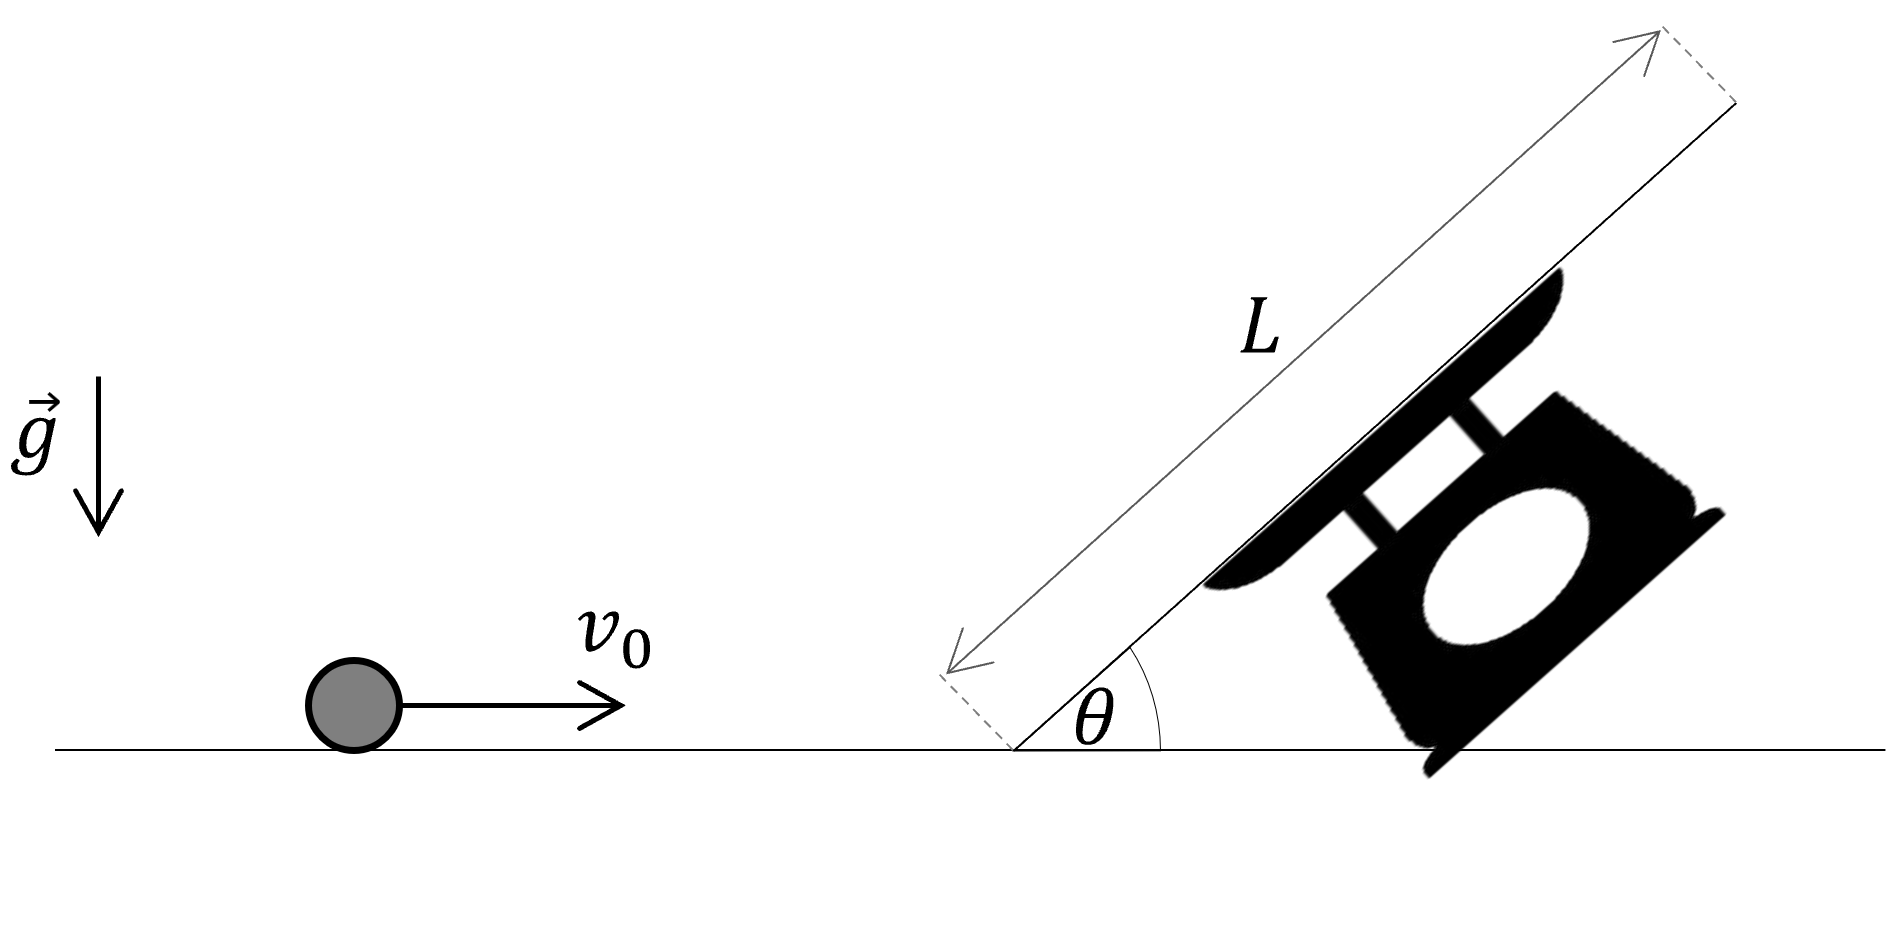
\includegraphics[width=0.4\linewidth]{2023-1/img/aux_5/balanza.png}
    \end{figure}
\end{enumerate}

\item 
\begin{multicols}{2}
Un estudiante de Introducción a la Física Clásica sección 1 se propone medir la aceleración que tiene un tren del metro al momento de salir de una estación. Para ello, ata una masa $m$ a un pasamanos utilizando una cuerda y con un transportador mide que el ángulo que forma la cuerda con el pasamanos es $\alpha$. Encuentre una expresión para determinar la aceleración buscada.
\columnbreak
\begin{figure}[H]
    \centering
    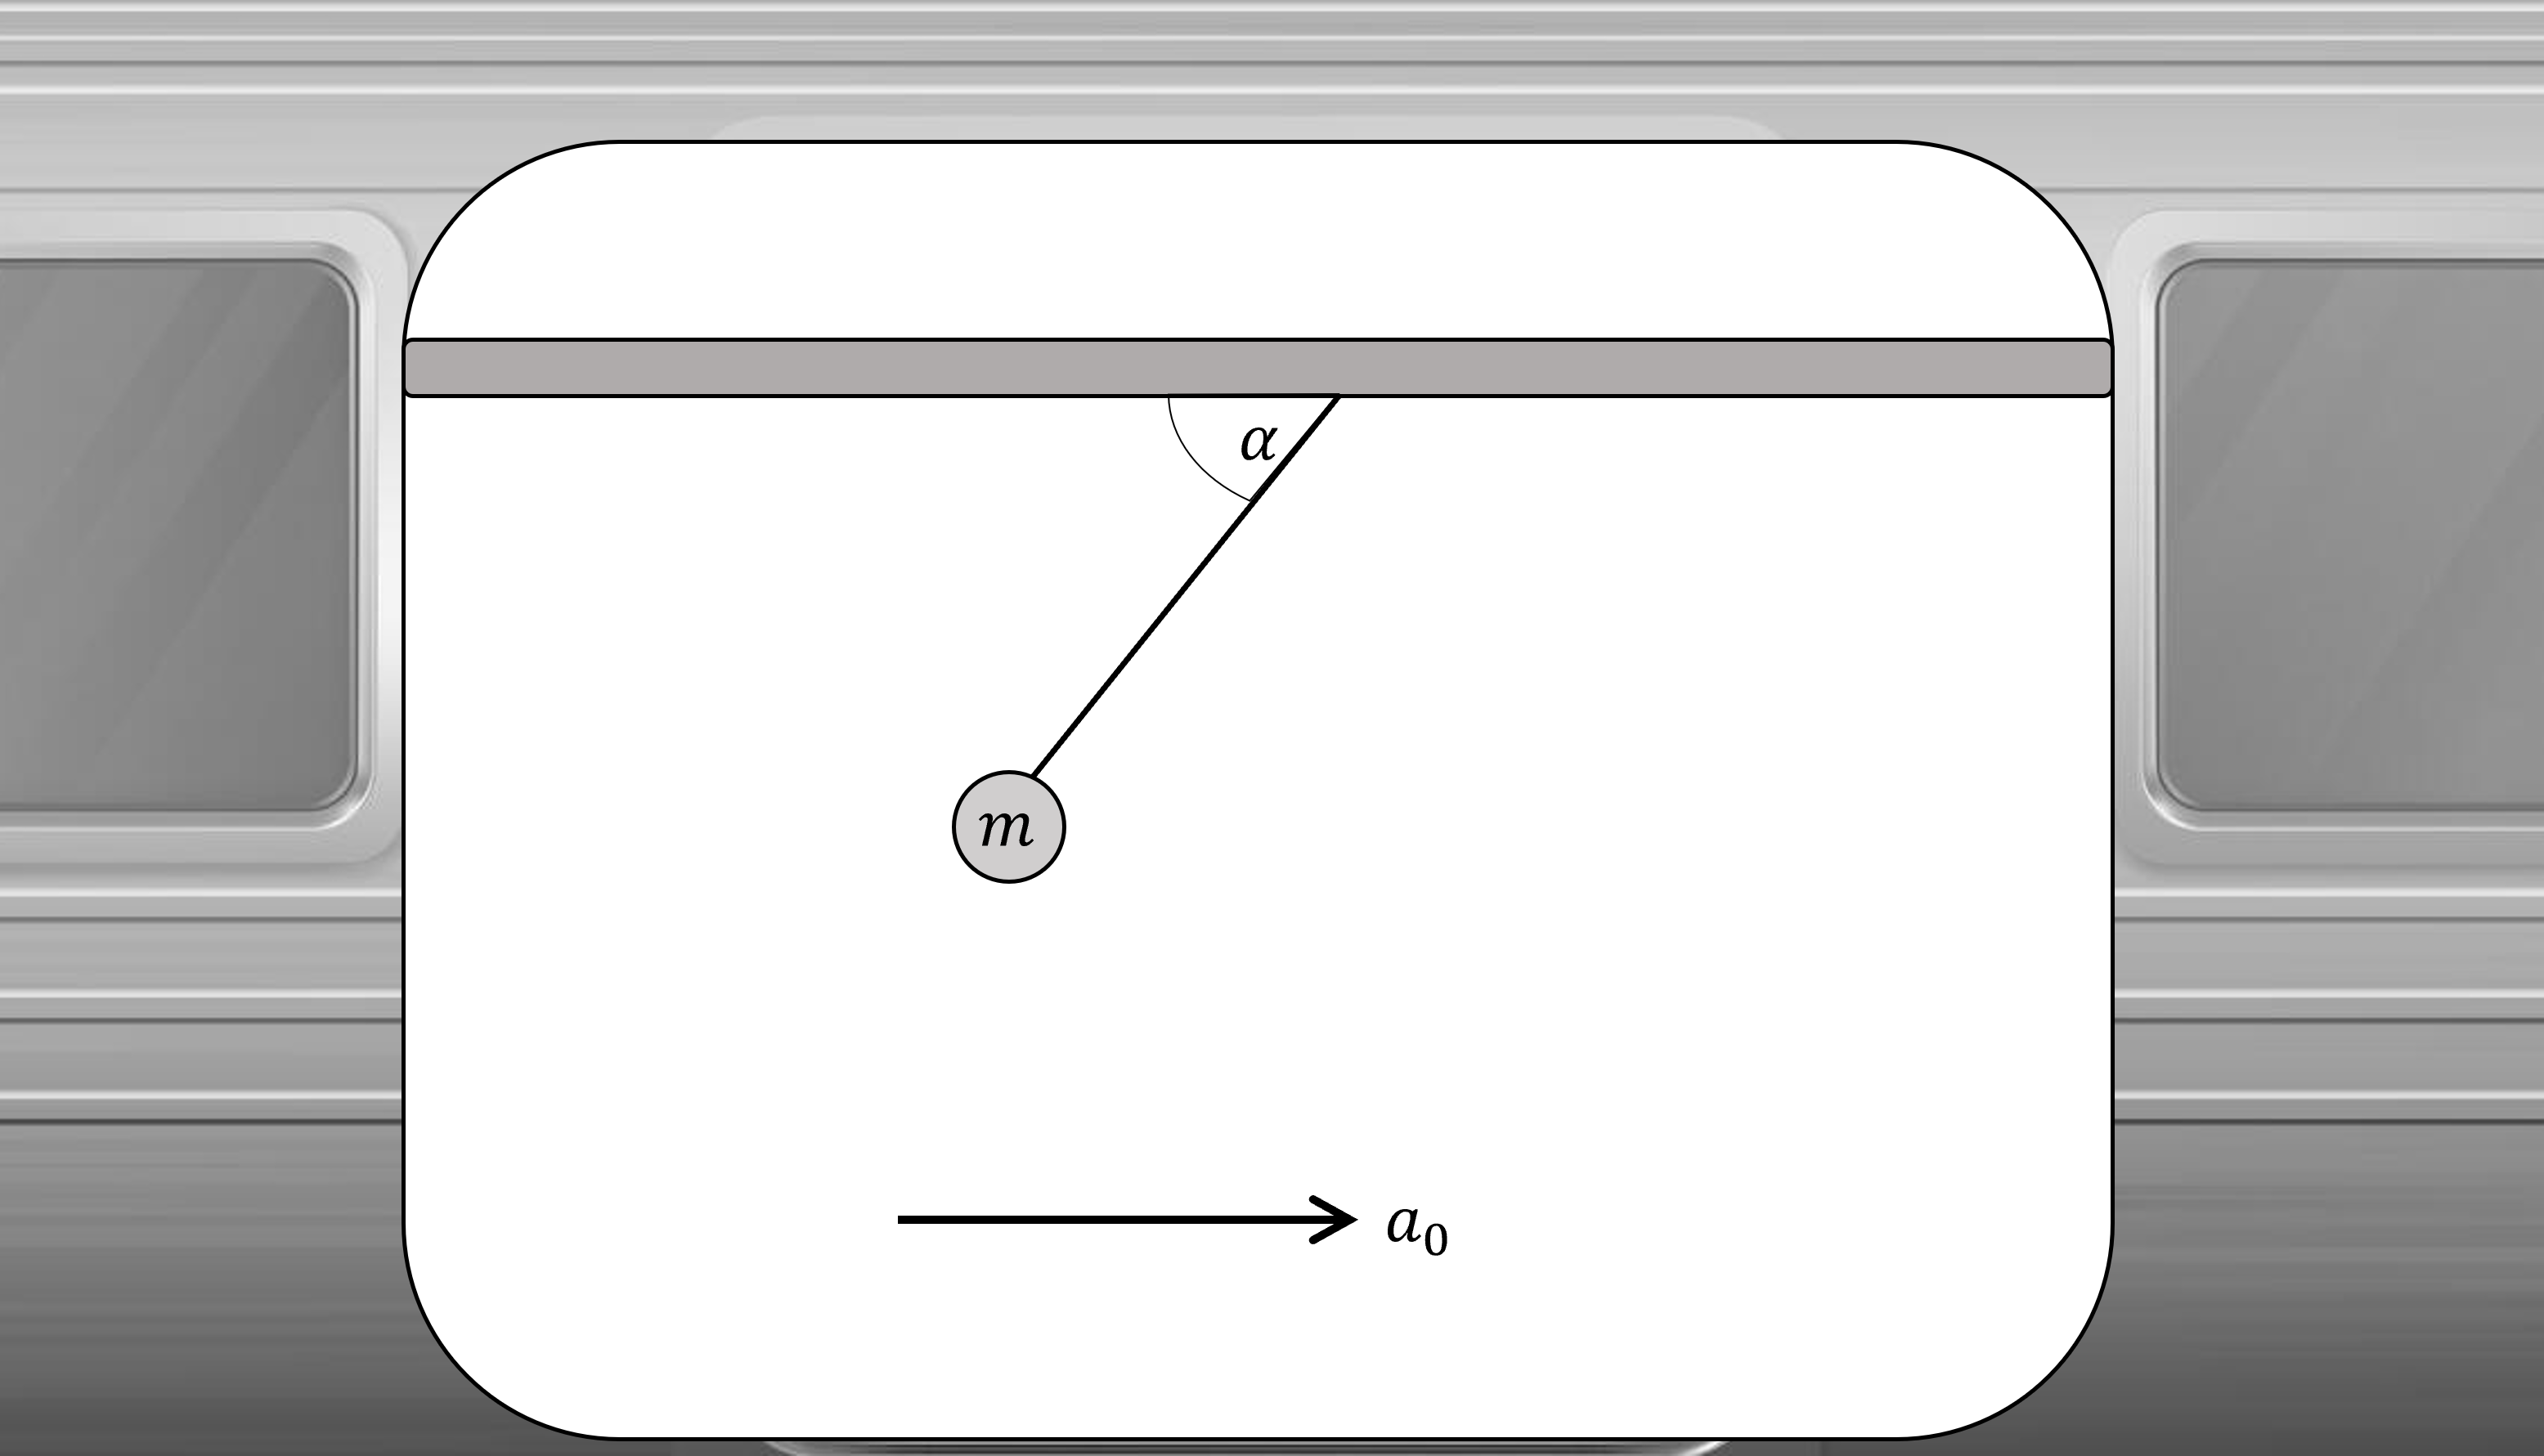
\includegraphics[width=0.8\linewidth]{2023-1/img/aux_5/metro.png}
\end{figure}
\end{multicols}

\item Una bolita de masa $m$ se encuentra rotando en la superficie de una esfera de radio $R$ con rapidez angular $\omega$. Si la bolita se encuentra atada a una cuerda, como se muestra en la figura, determine cuál es la rapidez angular mínima que la bolita debe tener para que la cuerda no se afloje.

\begin{figure}[H]
    \centering
    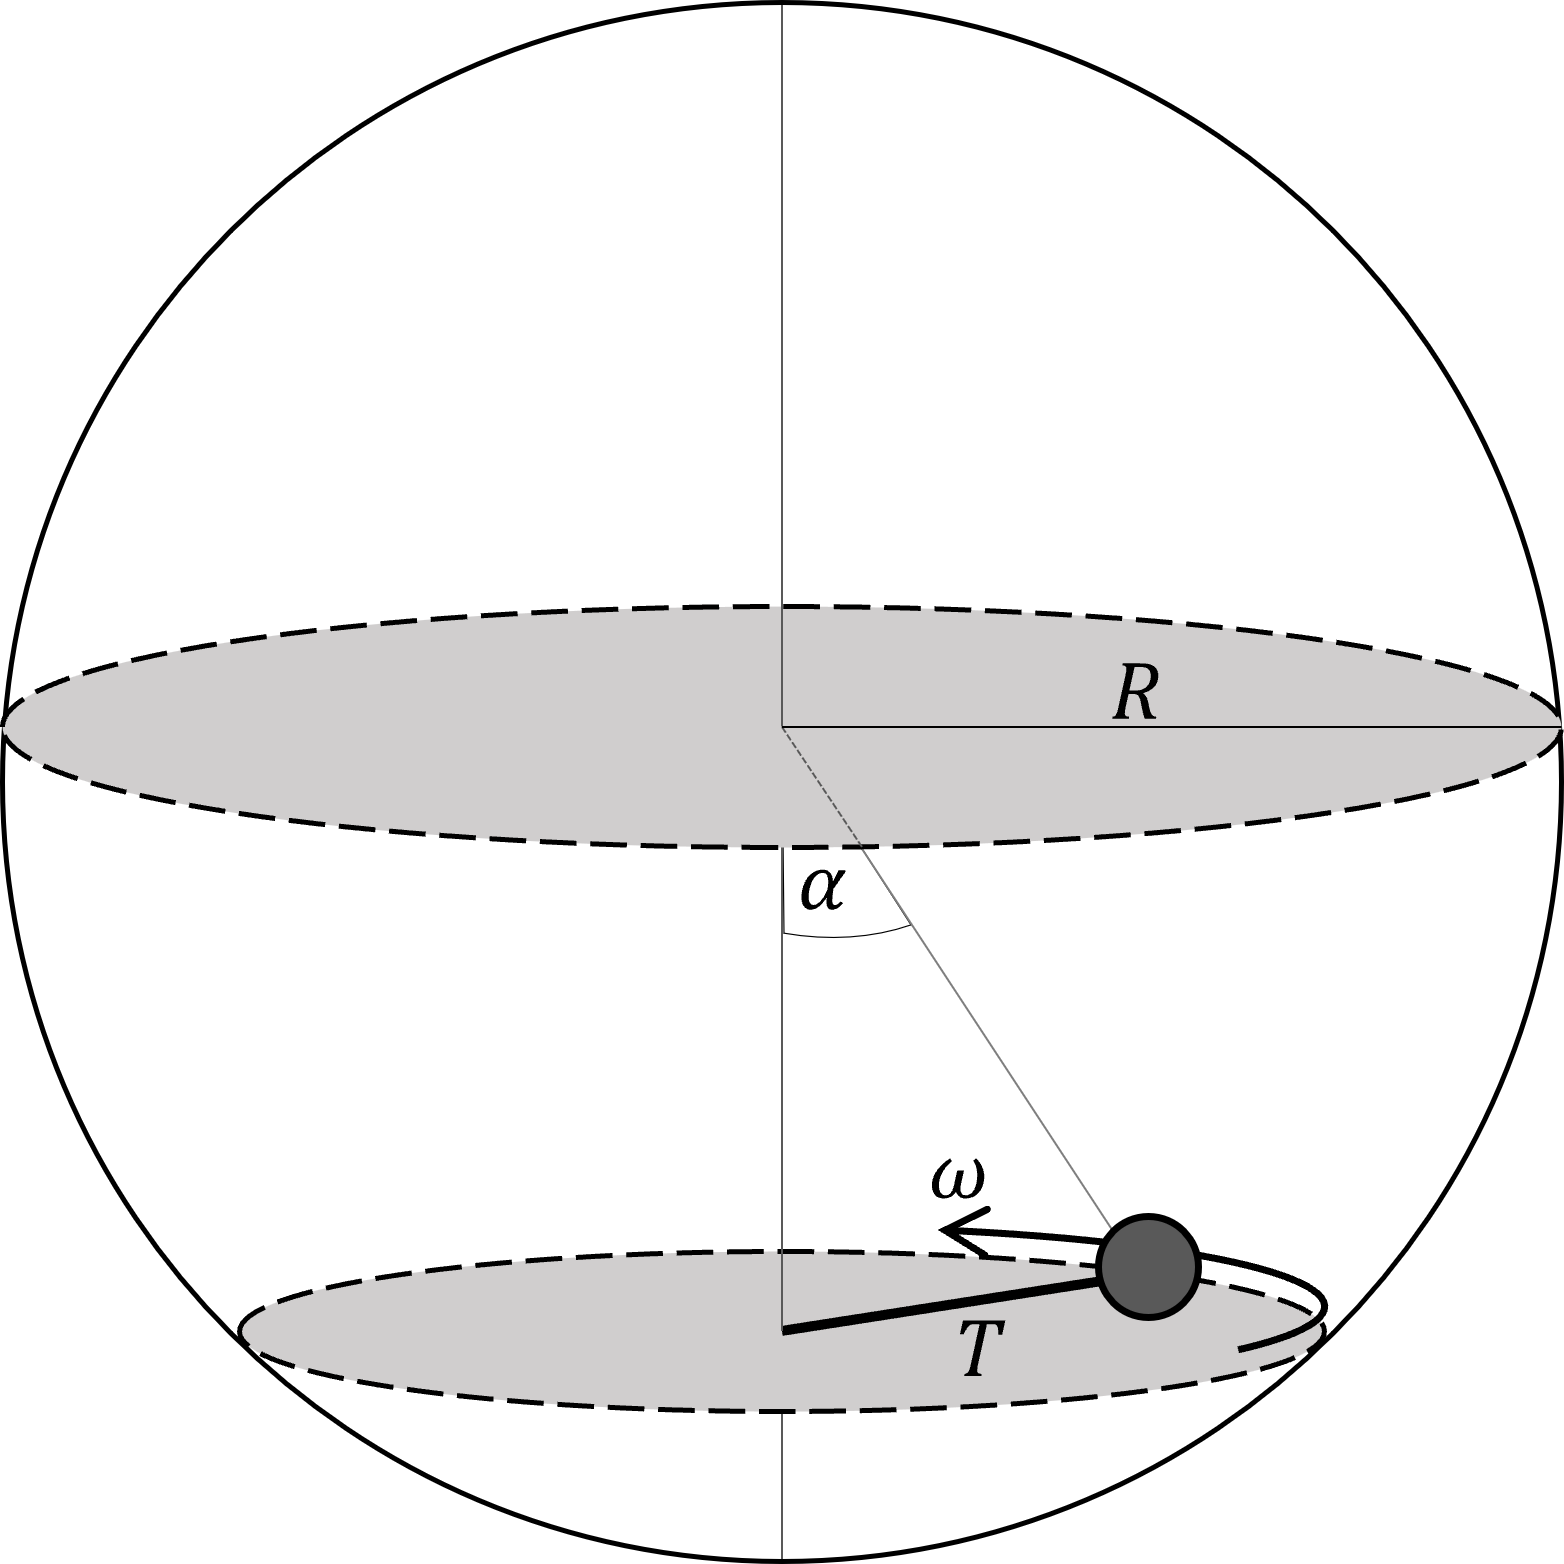
\includegraphics[width=0.3\linewidth]{2023-1/img/aux_5/esfera.png}
\end{figure}



% Para imágenes vectoriales -> el texto tiene que estar en LaTeX
% \begin{figure}[htbp]
%   \centering
%   \svgpath{../Imagenes/ejercicios}  -> .. irse pa'trás 
%   \includesvg{ej5.svg}
% \end{figure}

\end{enumerate}
\end{document}
